%%%%%%%%%%%%%%%%%%%%%%%%%%%%%%%%%%%%%%%%%%%%%%%%%%%%%%%%%%%%%%%%%%% 
%                                                                 %
%                            CHAPTER                              %
%                                                                 %
%%%%%%%%%%%%%%%%%%%%%%%%%%%%%%%%%%%%%%%%%%%%%%%%%%%%%%%%%%%%%%%%%%% 

\chapter{Platforms for accelerating the Smith-Waterman algorithm}
\label{ch:Platforms}

As we have discussed in Subsection~\ref{expl:SWanalyse} (analysis of the Smith-Waterman algorithm) the value of each cell in the matrix is only dependent on the left-upmost 3 cells. Therefore, it leads us to believe that this algorithm can be accelerated on other hardware solutions that are better equipped for parallelism than a normal CPU.

\section{Overview of possible hardware}

When designing a processing unit based on the semiconductor technology, it is always a tradeoff between efficiency and flexibility. For example, the CPU in a PC is highly flexible so that it can run any set of instructions without a lot of intervention between context changes. On the other hand, if a certain algorithm or instruction set should be executed as fast as possible, the FPGA's and ASICs are the best choices. At the extreme, an ASIC or \emph{Application Specific Integrated Circuit} can be chosen, but this means a complete chip should be designed from scratch just for this specific application. However, an ASIC is extremely expensive to design and build, especially for small production quantities. In figure~\ref{fig:effVSflex} an overview of the different options can be found.

\begin{figure}[H]
	%src=https://docs.microsoft.com/en-us/azure/machine-learning/service/media/concept-accelerate-with-fpgas/azure-machine-learning-fpga-comparison.png
	\centering
	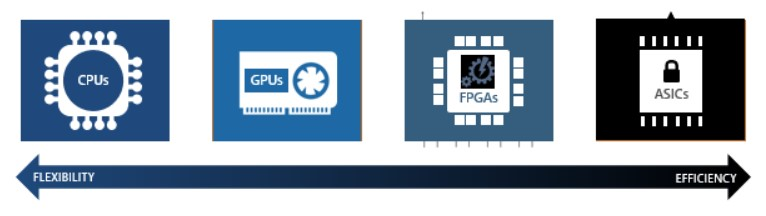
\includegraphics[width=0.75\textwidth]{elBackground/effVSflex.jpg}
	\caption{An overview of the different semiconductor technologies~\cite{fpgacomparison}.}
	\label{fig:effVSflex}
\end{figure}

\subsection{CPU}

The power of the CPU lies in its flexibility: it can be very easily programmed with new instructions in a short time. However, if the CPU would only run one specific algorithm for its whole lifetime, it would be terribly inefficient. Also, CPUs work sequentially, which is less suitable for algorithms that demand a large number of computations which could be done in parallel.

\begin{figure}[H]
	%src=http://www.lighterra.com/papers/modernmicroprocessors/sequential2.png
	\centering
	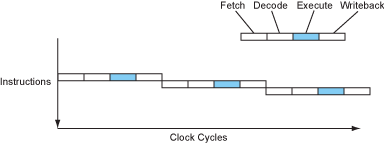
\includegraphics[width=0.75\textwidth]{elBackground/CPU.png}
	\caption{A cpu processes instructions sequentially. It could be accelerated using pipelining, but the maximum stays 1 instruction per clock cycle~\cite{Lighterra}.}
	\label{fig:cpu}
\end{figure}

Since the original implementations of the S-W algorithm are on a CPU, it became clear that a CPU was not the most suitable platform since it consists of a lot of operations that can be done in parallel. However, since the rise of SIMD, CPU's speed for parallel operations have improved substantially. \emph{SIMD} stands for \emph{Single Instruction Multiple Data} and makes it possible to manipulate more than 1 attribute of data with a single instruction, although it is the same instruction on all the data. CLC bio, a Danish company specialized in bioinformatics, has been able to achieve impressive speedups with a software implementation using SIMD, closing in on 200x~\cite{CLCbio}.
%src:https://web.archive.org/web/20070811101052/http://www.clccell.com/download.html

\subsection{GPU}

A GPU or \emph{Graphical Processing Unit} is a semiconductor technology which is specialized in video encoding and decoding. Since video encoding and decoding are actually glorified matrix manipulations, a GPU could also be used to manipulate all kinds of matrices. Since the Smith-Waterman algorithm is a big matrix fill in, it leads researchers to believe that it could be accelerated on a GPU. In 1997, an implementation of S-W on a GPU was published which achieved a speedup of 2x over all previous software implementations~\cite{gpuImpl}.
%src:  https://archive.org/details/computationalsci0000iccs_y9o8/page/230

\subsection{FPGA}

An FPGA, or \emph{Field Programmable Gate Array}, is an integrated circuit consisting of programmable logic components. These logic components can be programmed as any logic function, such as an AND, XOR, etc. In most FPGA other elements are also found, such as memory blocks, DSP blocks, etc.

Most basic FPGA's, containt the following items:
\begin{enumerate}
	\item CLB's, or \emph{Complex Logic Blocks}, consisting of a \emph{LookUp Table} (LUT) and a flipflop. A LUT can be programmed so that it contains any type of logic function.
	\item Programmable Interconnects have to connect the CLB's into a bigger circuit, which is also called \emph{routing}. This routing has the most influence on delays, and are also responsible for most errors.
	\item I/O blocks, which connect the internal logic inside with the outside pins of the FPGA. Most can be configured as input, output, or bidirectional.
\end{enumerate}

\begin{figure}[H]
	%src=https://evergreen.loyola.edu/dhhoe/www/FPGA_diagram.png
	\centering
	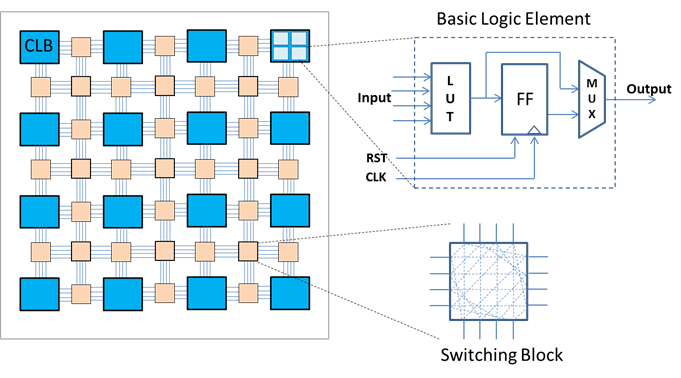
\includegraphics[width=0.75\textwidth]{elBackground/FPGA.png}
	\caption{The basic layout of an FPGA~\cite{fpgaworkings}.}
	\label{fig:fpga}
\end{figure}

For an implementation or design of a circuit which should be loaded in an FPGA, a \emph{Hardware Description Language} (HDL) is often the only practical choice to implement such a system, since drawing the circuits with a CAD program or by hand would take a very long time.

In a paper from 2007, an implementation of S-W with an FPGA (Virtex-4) achieved a speedup of up to 100x in comparison with a 2.2GHz Opteron processor~\cite{fpga100x}.%src https://ft.ornl.gov/~olaf/pubs/RSSIOlafDave.pdf
A few companies have also made some implementations on FPGA in the past, e.g. Cray Inc.~\cite{Cray}, TimeLogics~\cite{Timelogics}, ...
%cray: https://www.cray.com/
%timelogics: http://www.timelogic.com/

A master's thesis from 2011 by Vermij E.~\cite{Vermij} %cit
 has a detailed analysis of an FPGA based Smith-Waterman implementation. In other~\cite{FPGAeff} papers, it was found that the performance per Watt level for an FPGA implementation is better than a GPU or CPU by a factor of 12-21 times.

\section{Hardware selection}

As the hardware the ZCU 104 evaluation kit was selected, which has an MPSoC onboard. An MPSoC (or \emph{Multi-Processor System on Chip}) is an integrated circuit that contains multiple microprocessors. This means that both a processor and programmable hardware is available.

\begin{figure}[H]
	\centering
	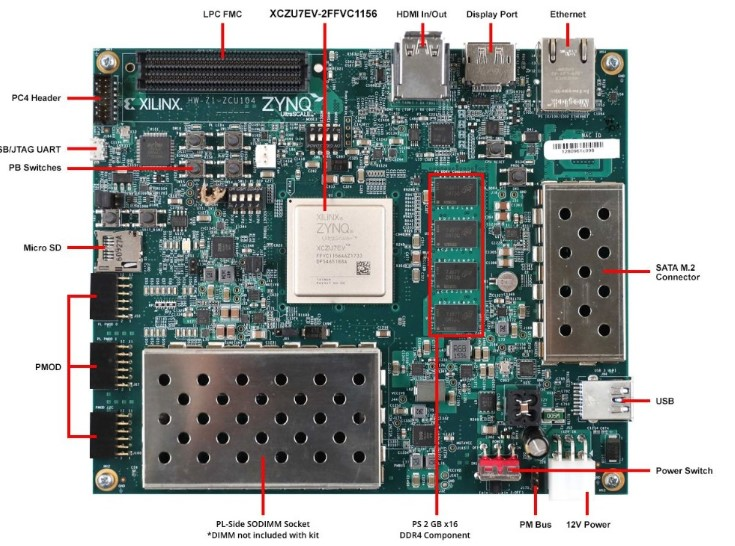
\includegraphics[width=0.75\textwidth]{elBackground/hardware.jpg}
	\caption{An overview of the hardware available on the ZCU 104 MPSoC evaluation kit}
	\label{fig:hardware}
\end{figure}

Reasons for choosing the ZCU 104 evaluation kit:
\begin{enumerate}
	\item An MPSoC is present, which will be used to the host application;
	\item Both a USB and Ethernet interface is available, which makes it easy to communicate with the target board;
	\item An operating system can be run on the board (a Red Hat Linux distribution). This means we won't have to worry about implementing FAT or Ethernet stacks;
	\item 16 times 2 gigabytes of RAM is available, which can be useful when implementing big structures, like the alignment matrix;
	\item It was available at the Brno University of Technology.
\end{enumerate}

\subsection{Recent advances in High-Level Synthesis}

When programming an FPGA, an HDL is often used. However, if a specific implementation already exists in a programming language, it often has to be reimplemented from scratch in HDL to load it on the FPGA. Therefore people have been trying to make a compiler that compiles normal C code into HDL. This "compiler" is called HLS, or \emph{ High-Level Synthesis}. In recent years, HLS became popular as an alternative for designing and implementing a complex system that should be run on an FPGA.

During research in the known literature, no implementation using HLS for the Smith-Waterman algorithm was found. That's why we believe that this is still an unexplored area.

\subsection{Platform communication}

Initially, it seemed important that there is good communication between the board and the host to load and unload sequences since we didn't want the communication to become the bottleneck. However, when using S-W for genome mapping, this won't be an issue since the time it takes to map a read takes a lot longer than the time to transfer it.

In the end, no direct communication with the board was implemented. It seemed sufficient to just load the reads with the genome on an SD card, and insert this in the board. After the mapping process, the mapped reads are available on the same SD card. However, if this program would be used in practice, it doesn't seem practical to constantly change out the SD card. Therefore, another solution should be found. A possible solution could be using the Ethernet stack available as part of the OS, so we could easily use FTP for on and off loading from and to the board.

\section{HLS and SDSoC learning tools}
\label{ch:InitDiff}

\textit{Disclaimer: The purpose of this section is to show the learning tools I used to achieve a suitable implementation for the genome mapping problem. New programming techniques such as HLS and SDSoC were familiarized. This section might be less applicable if the reader is interested in the science and implementation approach of the genome mapping problem, but can be interesting if the reader is also new to the mentioned programming techniques.}

\subsection{Using Vivado HLS and Xilinx SDK}

\paragraph{Learning HLS in examples}
\label{HLS}

To learn HLS, I used learning materials sent to me by Tom\'a\v s Mart\'inek, who works at the Brno University of Technology~\cite{martinek}. It contains a theory part,  and also hands-on lab examples. These labs were worth exploring in this thesis since they contain most concepts of HLS.

\paragraph{Learning how to program target board}

At first, the Xilinx SDK was used to program the board. However, it was found to be unpractical to use, because after programming a "Hello World" application it became clear that the easiest way to program it this way would be bare-metal. Therefore, a FAT or Ethernet stack ourselves would need to be implemented.
Therefore the SDSoC IDE was used for programming the target board, which structures the application on top of an operating system. This operating system provides the Ethernet and FAT stacks.

\subsection{SDSoC}

SDSoC is an IDE developed by Xilinx which is specialized in programming MPSoCs. It is based on the Eclipse IDE, so most of its features are known by most programmers. 

The strength of SDSoC lays in the ability to easily transfer functions from software to programmable logic. It can be done with the click of a button. Then, the functions marked for hardware (written in C) will be fitted in the programmable logic using the HLS compiler. However, the syntax is not always accepted since HLS cannot implement every possible programming technique in C yet.

As mentioned earlier, in this implementation we will work on a Linux distribution.

\paragraph{Learning process on matrix multiplication example in SDSoC}

To learn MPSoC and the SDSoC IDE, Xilinx' online available materials were used, available at their GitHub page, which includes some hands-on assignments. The assignments use a matrix multiplication example, preinstalled with SDSoC. A weblink to this GitHub page can be found in the references~\cite{sdsoc}.

